\begin{figure}[!h]
    \centering
    \begin{subfigure}{.5\textwidth}
      \centering
      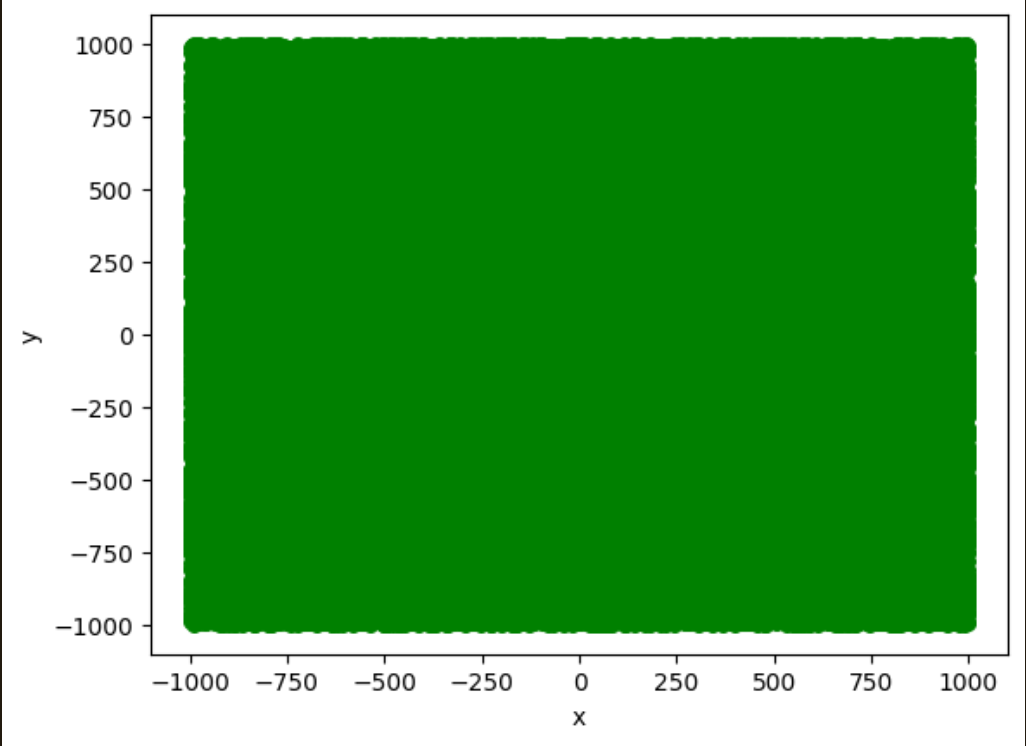
\includegraphics[width=.9\linewidth]{1.png}
      \caption*{Rys. 1: (a) $10^5$ losowych punktów $(x, y) \in \left[-1000,1000\right]^{2}$.}
      \label{fig:sub1}
    \end{subfigure}%
    \begin{subfigure}{.5\textwidth}
      \centering
      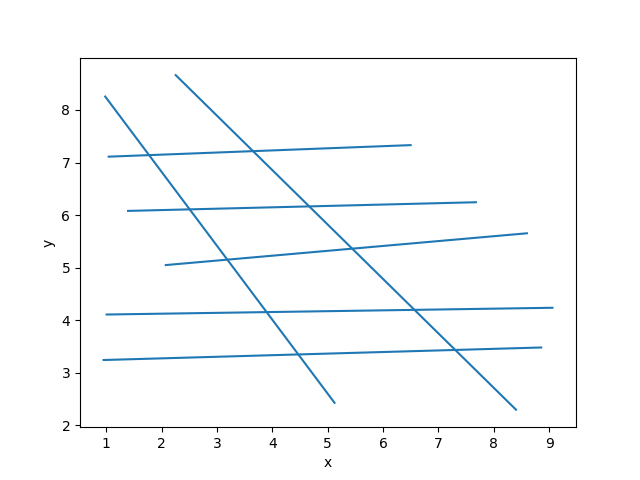
\includegraphics[width=.9\linewidth]{2.png}
      \caption*{Rys. 2: (b) $10^5$ losowych punktów $(x, y) \in \left[-10^{14},10^{14}\right]^{2}$.}
      \label{fig:sub2}
    \end{subfigure}
    \label{fig:test}
    \end{figure}
    \begin{figure}[!h]
    \centering
    \begin{minipage}{.5\textwidth}
      \centering
      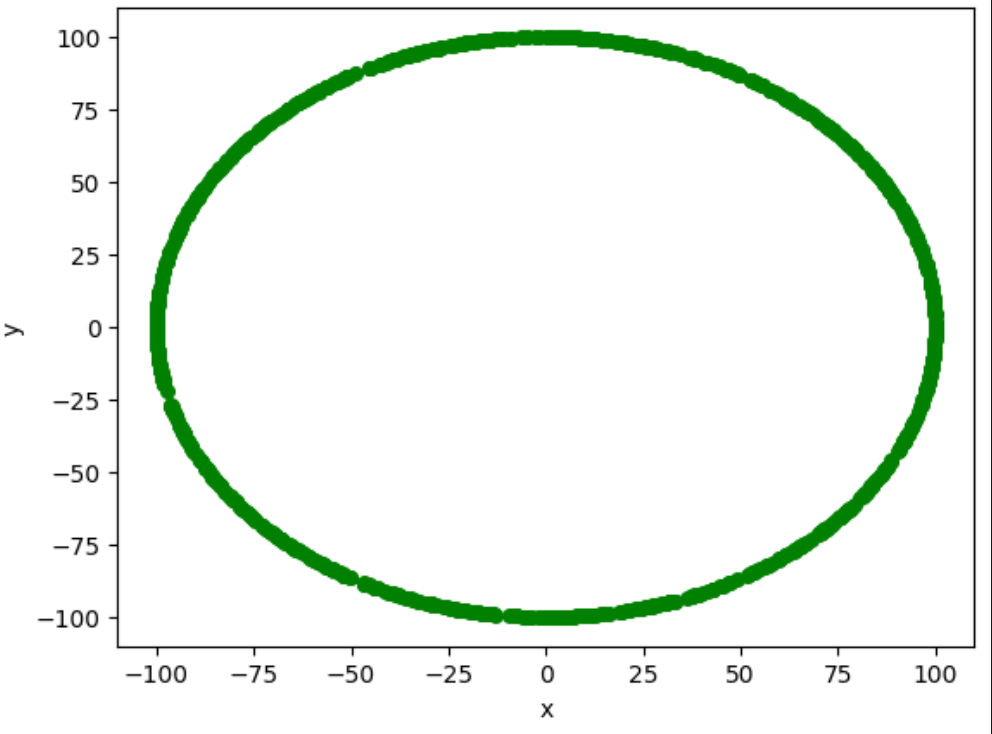
\includegraphics[width=.9\linewidth]{3.png}
      \caption*{Rys. 3: (c) $1000$ losowych punktów leżących na okręgu.}
      \label{fig:test1}
    \end{minipage}%
    \begin{minipage}{.5\textwidth}
      \centering
      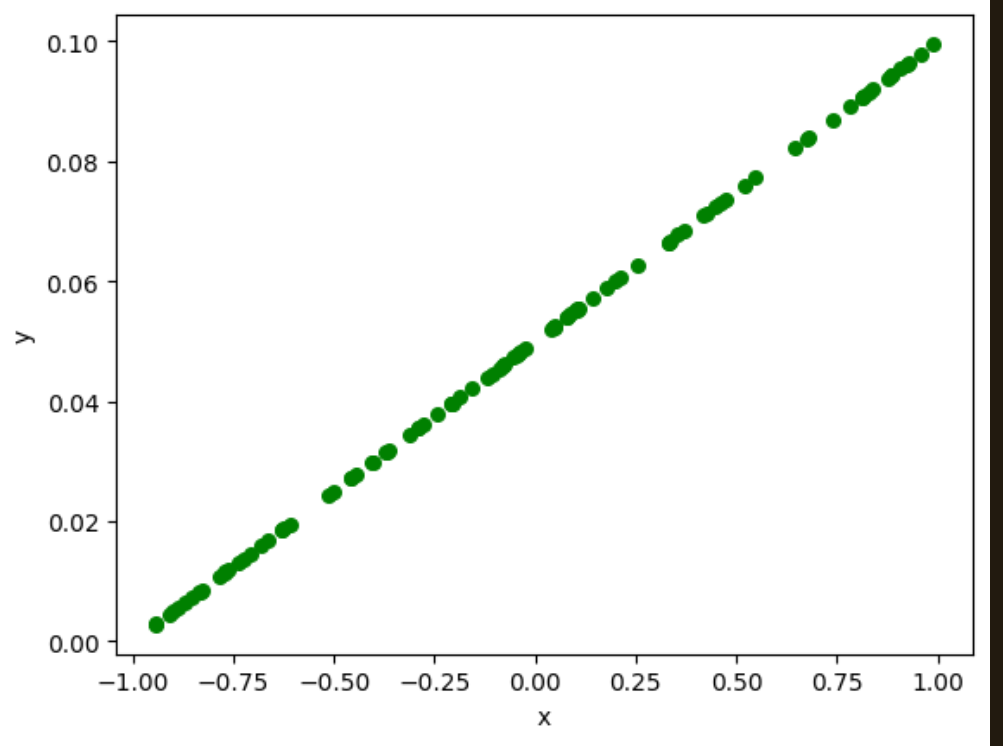
\includegraphics[width=.9\linewidth]{4.png}
      \caption*{Rys. 4: (d) $1000$ losowych punktów na prostej.}
      \label{fig:test2}
    \end{minipage}
    \end{figure}
\null
    \subsection{Algorytmy generacji zbiorów}
    \begin{enumerate}
    \item Dla zbiorów a i b. Osobna generacja każdego z $10^5$ losowych punktów.
    \item Dla zbioru c. Parametryzacja punktów na okręgu za pomocją funkcji trygonometrycznych $\sin$ i $\cos$.
    \item Dla zbioru d. Przekształcenie odcinka do postaci parametrycznej 
    $$
    l:\begin{cases}
      x = x_0 + tv_x& \smash{\raisebox{-1.6ex}{dla $\boldsymbol t \in [0,1]$.}}\\
      y = y_0 + tv_y
    \end{cases}
    $$
    A potem generowanie $t$ w podanym przedziale i dodanie odpowiednich punktów.
    \end{enumerate}
% \newpage